\svnid{$Id: plot_styles.tex 80815 2026-02-17 17:10:15Z jagers $}

\chapter{Plot styles} \label{Chp:PlotStyles}
At the end of `Getting started' chapter, we created a map plot, a line graph of along a cross section, and a line graph of a time series.
Depending on the quantities selected, \QUICKPLOT can create various other plots.
This chapter describes the various plot types

\begin{itemize}
\item 1D graph of a scalar time series (\Sref{Subsec:GraphTimeSeriesScalar}),
\item 1D graph of a 2D quantity along a transect (\Sref{Subsec:GraphTransectScalar2D}),
\item 1D graph of a 3D quantity along a profile (\Sref{Subsec:GraphProfileScalar3D}),
\item 2D map plot of a scalar quantity (optionally a 2D horizontal slice of 3D quantity) (\Sref{Subsec:MapScalar}),
\item 2D map plot of a vector quantity (optionally a 2D horizontal slice of 3D quantity) (\Sref{Subsec:MapVector}),
\item 2D map plot of tracks (\Sref{Subsec:MapTracks}),
\item 2D vertical slice of a 3D quantity (\Sref{Subsec:SliceScalar}),
\item 2D side of 3D tracks (\Sref{Subsec:VerticalTracks}),
\item 2D vertical profile plotted against time (\Sref{Subsec:ProfileTime}),
\item 2D surface in 3D (\Sref{Subsec:2DSurfaceIn3D}),
\end{itemize}

%------------------------------------------------------------------------------
\section{Graphs} \label{Sec:PlotStyleGraph}

\subsection{Graph of a scalar time series} \label{Subsec:GraphTimeSeriesScalar}
The most common line graph is a time-series plot showing the variation of a quantity along the vertical axis over time plotted along the horizontal axis.
They are great for visualizing the time response of a system at one or more characteristic locations.
If the quantity is an elevation, such as the water level or the bed level, the vertical co-ordinate (elevation) is used along the vertical axis.
In that case we can also add the time variation of a profile to the same graph (see \Autoref{Subsec:ProfileTime}).
For all other quantities the quantity itself is plotted along the vertical axis.
Line styles and markers can be used to identify different lines when plotted in one graph.
By setting the axes type equal to ``Time'' for a quantity, you can add a vertical line at a specific time to a time series graph.
This line can be animated together with a map or cross-section in another graph.

\begin{figure}[H]
\center{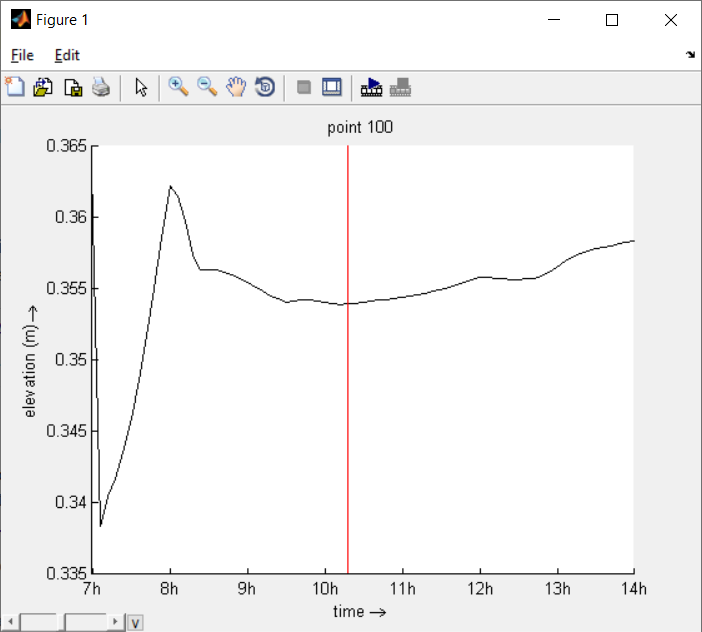
\includegraphics[width=100mm]{Ch06/TimeSeriesLine.png}}
\caption{Time series plot of the water levels at point 100 with a time marker.}
\label{fig:TimeSeriesLine}
\end{figure}

\subsection{Graph of a 2D quantity along a transect} \label{Subsec:GraphTransectScalar2D}
Another common line graph is a cross-section plot showing the variation of a quantity along the vertical axis over a distance plotted along the horizontal axis.
Although the title of this section refers to a transect, you may think of any arbitrary path across the stream, along a stream, or along any other line.
If the quantity is an elevation, such as the water level or the bed level, the vertical co-ordinate (elevation) is used along the vertical axis.
In that case we can also add other vertical slices to the same graph (see \Autoref{Sec:PlotStyleSlices}).
For all other quantities the quantity itself is plotted along the vertical axis.

\subsection{Graph of a 3D quantity along a profile} \label{Subsec:GraphProfileScalar3D}
The vertical variant of the transect is the profile plot: the variation of a quantity is plotted along the horizontal axis over a range of vertical co-ordinates plotted along the vertical axis.

%------------------------------------------------------------------------------
\section{Map Plots - including horizontal slices} \label{Sec:PlotStyleMaps}
A map plot is characterized by a 2D graph of a quantity in a ``horizontal'' plane (the two plot directions represent X and Y co-ordinates, or longitude and latitude).
The quantity plotted may be any 2D quantity or a ``horizontal'' slice of a 3D quantity.
In this context we use the term ``horizontal'' slice to refer to any slice  through a 3D quantity that returns a unique value for every point in the horizontal plane -- this can be slice at a specific Z value or at a specific fraction of the water depth (commonly referred to as $\sigma$-plane) or any similar ``horizontal'' plane (see Section \ref{Subsec:SliceScalar} on vertical slices along a line).
As shown in Figure \ref{fig:HSliceOptionsList}, the program currently supports five ways of creating a ``horizontal'' slice

\begin{figure}[H]
\center{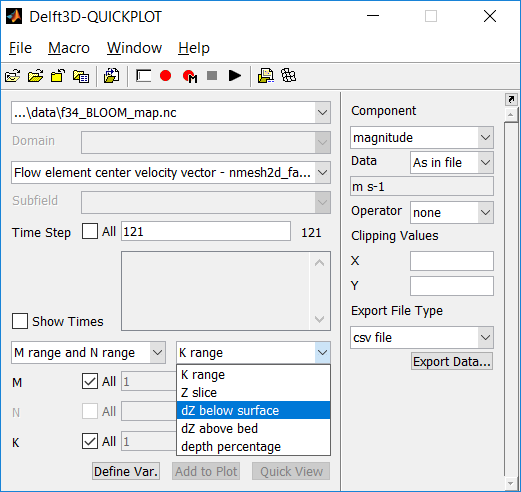
\includegraphics[width=100mm]{Ch06/HSliceOptionsList.png}}
\caption{List of five horizontal slicing options.}
\label{fig:HSliceOptionsList}
\end{figure}

\begin{itemize}
\item Selecting a model layer (K-value; elevation may vary depending on the model)
\item Selecting a plane at a fixed elevation (Z-value, typically in m above the reference plane of the model; elevation doesn't change)
\item Selecting a plane at a fixed height below the surface (dZ-value, typically in m; elevation changes if the surface elevation changes)
\item Selecting a plane at a fixed height above the bed (dZ-value, typically in m; elevation changes if the bed level changes)
\item Selecting a plane at a fixed percentage of the water depth (measured from the surface (0 \%) to bed (100 \%)).
\end{itemize}

\subsection{Map plot of a scalar field} \label{Subsec:MapScalar}
The default map plot type for a 2D scalar field defined on a mesh is the patches plot.
Figure \ref{fig:HSliceScalarPatches} shows an example of the velocity magnitude along a plane at 0.5 m below the water surface.
Other presentation types supported include

\begin{figure}[H]
\center{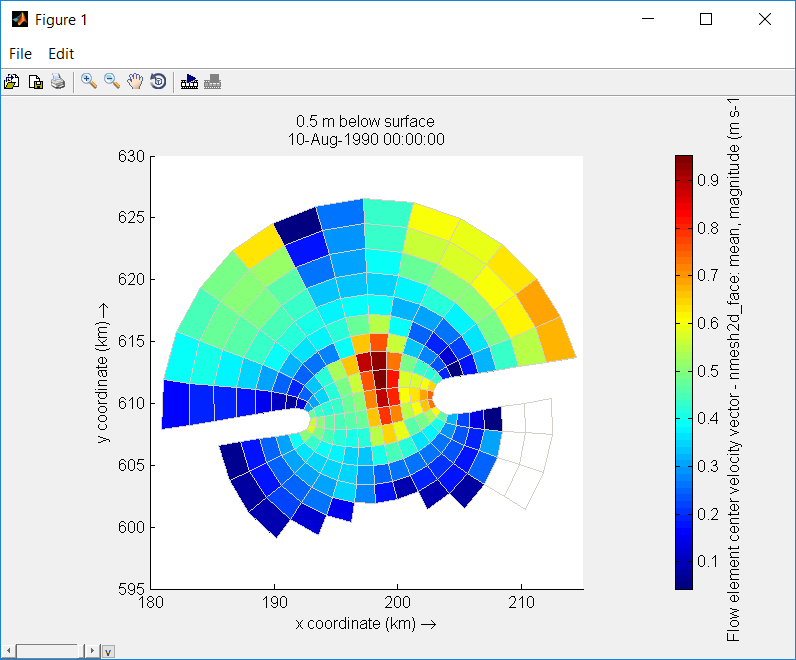
\includegraphics[width=100mm]{Ch06/HSliceScalarPatches.png}}
\caption{Patches plot of a ``horizontal'' slice of the flow velocity.}
\label{fig:HSliceScalarPatches}
\end{figure}

\begin{itemize}
\item patches: this plot style fills each grid cell with a uniform colour based on the value within that grid cell.
\item patches with lines: same as the default patches plot, but also highlighting the grid cell edges with lines.
\item markers: a marker is plotted at each data location instead of filling the whole grid cell.
The colour of the marker usually depends on the value.
\item values: a number is plotted at each data location instead of marker.
This plot option is slow for large numbers of values (use the dynamic field thinning option to work smoothly with large value fields).
\item continuous shades: the values are interpolated in between the data locations to generate smooth colour transitions.
\item contour lines: contour lines are drawn based on the interpolated data values.
The contour lines have a uniform colour.
\item coloured contour lines: same as `contour lines' but in this case each contour line is coloured based on the value that corresponds to that line.
\item contour patches: the areas between the contour lines are filled with a uniform colour; the contour lines themselves are not drawn explicitly.
\item contour patches with lines: same as `contour patches' but in this case also the contour lines are drawn in a uniform colour.
\item edges: if the data is defined at the edges of the mesh, each edge may be coloured based on the local value.
\item polygons: if the data is not defined on a mesh, but on a set of polygons such as a GIS coverage, each polygon may be coloured based on the associated value (similarly to the default `patches' plot for gridded data).
\end{itemize}

The available options for the presentation type depend on the location at which the data is defined, not on the way in which the data was obtained i.e.~a horizontal slice of a 3D quantity can be plotted in exactly the same ways as any 2D quantity.

\subsection{Map plot of a vector field} \label{Subsec:MapVector}
The main additional map plot type supported for simulation data is the vector plot.
The vectors may be drawn using a uniform colour, or coloured based on the value of one of its components.
Alternatively, you may select a scalar component (including magnitude and various definitions of the angle) and plot that component as a scalar quantity.

\subsection{Map plot of tracks} \label{Subsec:MapTracks}
Particles (or surface drogues) are transported by the wind, waves, and currents.
Such objects (sometimes referred to as individuals or agents) are characterized by pathways or tracks of their position as function of time: $x(t)$, $y(t)$ and optionally $z(t)$.
Not just their position, but also their properties may vary over time.
\QUICKPLOT\ can visualize these tracks as lines (either using a uniform colour, or shaded by some property e.g.~time or vertical co-ordinate), or animate their position using a field of markers.

\subsection{Horizontal transect against time} \label{Subsec:TransectTime}
A less common, but sometimes very informative 2D plot shows the development over time of a quantity along a transect (or other arbitrary path).
The basic concept is the same as for the line graph discussed in \Autoref{Subsec:GraphTransectScalar2D}, but extended with the time-dimension.
Instead of creating an animation of the line graph, the variation of the quantity is captured by the colours of a 2D map of which one axis marks the distance along the path, and the other axis indicates the variation over time.
The `patches' and `patches with lines' presentation types are not yet available for these plots.

%------------------------------------------------------------------------------
\section{Vertical slice plots} \label{Sec:PlotStyleSlices}
This is the vertical version of the 2D map plots described in \Autoref{Sec:PlotStyleMaps}.
In this case the vertical axis in the plot corresponds with the vertical co-ordinate in the data.
The horizontal axis is typically a horizontal co-ordinate, but it can also indicate time.

\subsection{Vertical slice of a 3D quantity} \label{Subsec:SliceScalar}
A vertical slice of a 3D quantity is characterised by the selection of a transect and multiple layers.
The most common way of selecting a transect is by means of an Arbitrary (x,y) Line, but an ordered list of aligned grid cells/nodes may also be used to identify the path.
As for the map plots of scalar quantities, the user may select different presentation types for vertical slices (see the full list of presentation types given in \Autoref{Subsec:MapScalar} -- only the `polygons' cannot be used for vertical slices).
The figures \ref{fig:VSliceScalarPatches} and \ref{fig:VSliceScalarContours} show a slice of the same quantities (velocity magnitude, water level, bed level) using two different presentation types.
The former figure is created using Patches for the slice of the 3D velocity magnitude and Stepwise for the slices of the 2D water level and bed level quantities.
The latter figure is created using Contour Patches for the velocity and Linear for the water level and bed level.
Both figures include vertical dotted lines which indicate the borders of the grid cells (plotted by means of the mesh topology variable).
The path of the slice and the model grid is shown for reference in \Fref{fig:VSliceScalarGridViewArbLine}; all quantities plotted are defined in the cells/faces.

\begin{figure}
\center{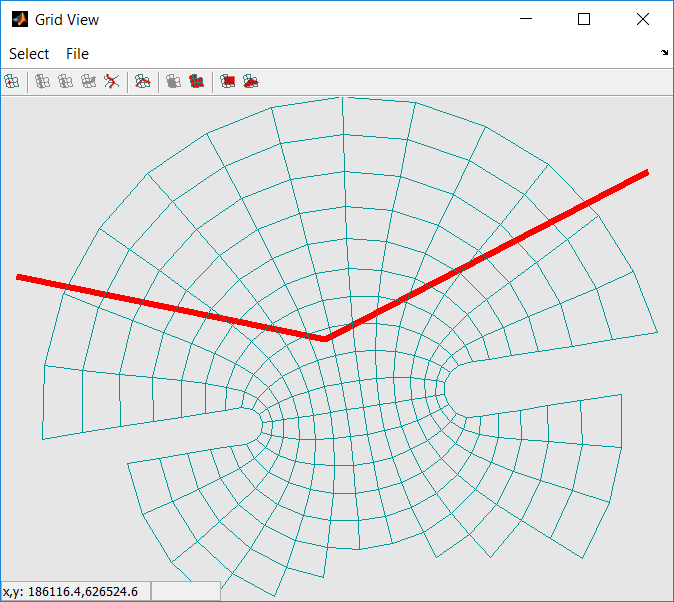
\includegraphics[width=100mm]{Ch06/VSliceScalarGridViewArbLine.png}}
\caption{Example of an arbitrary line slicing through an unstructured grid.}
\label{fig:VSliceScalarGridViewArbLine}
\end{figure}

\begin{figure}
\center{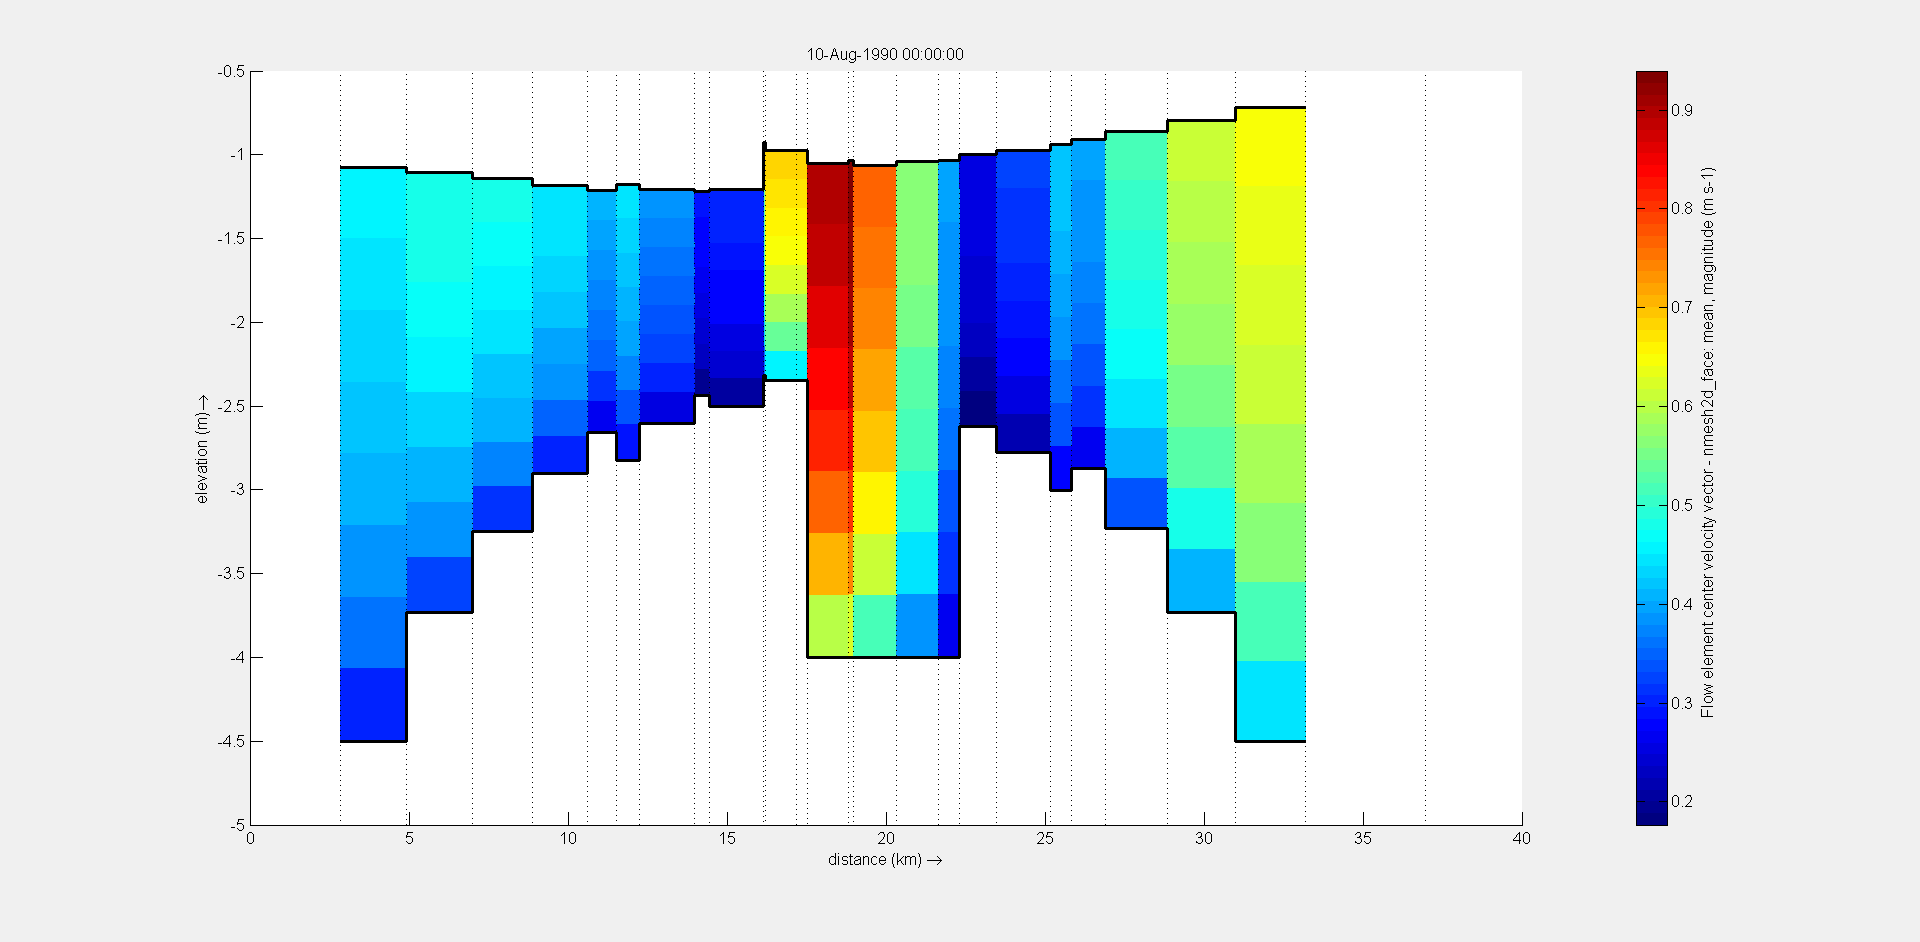
\includegraphics[width=\textwidth]{Ch06/VSliceScalarPatches.png}}
\caption{Slice of the velocity magnitude along the line shown in \Fref{fig:VSliceScalarGridViewArbLine} using presentation type Patches for the velocity and Stepwise for the water level and the bed level.}
\label{fig:VSliceScalarPatches}
\end{figure}

\begin{figure}
\center{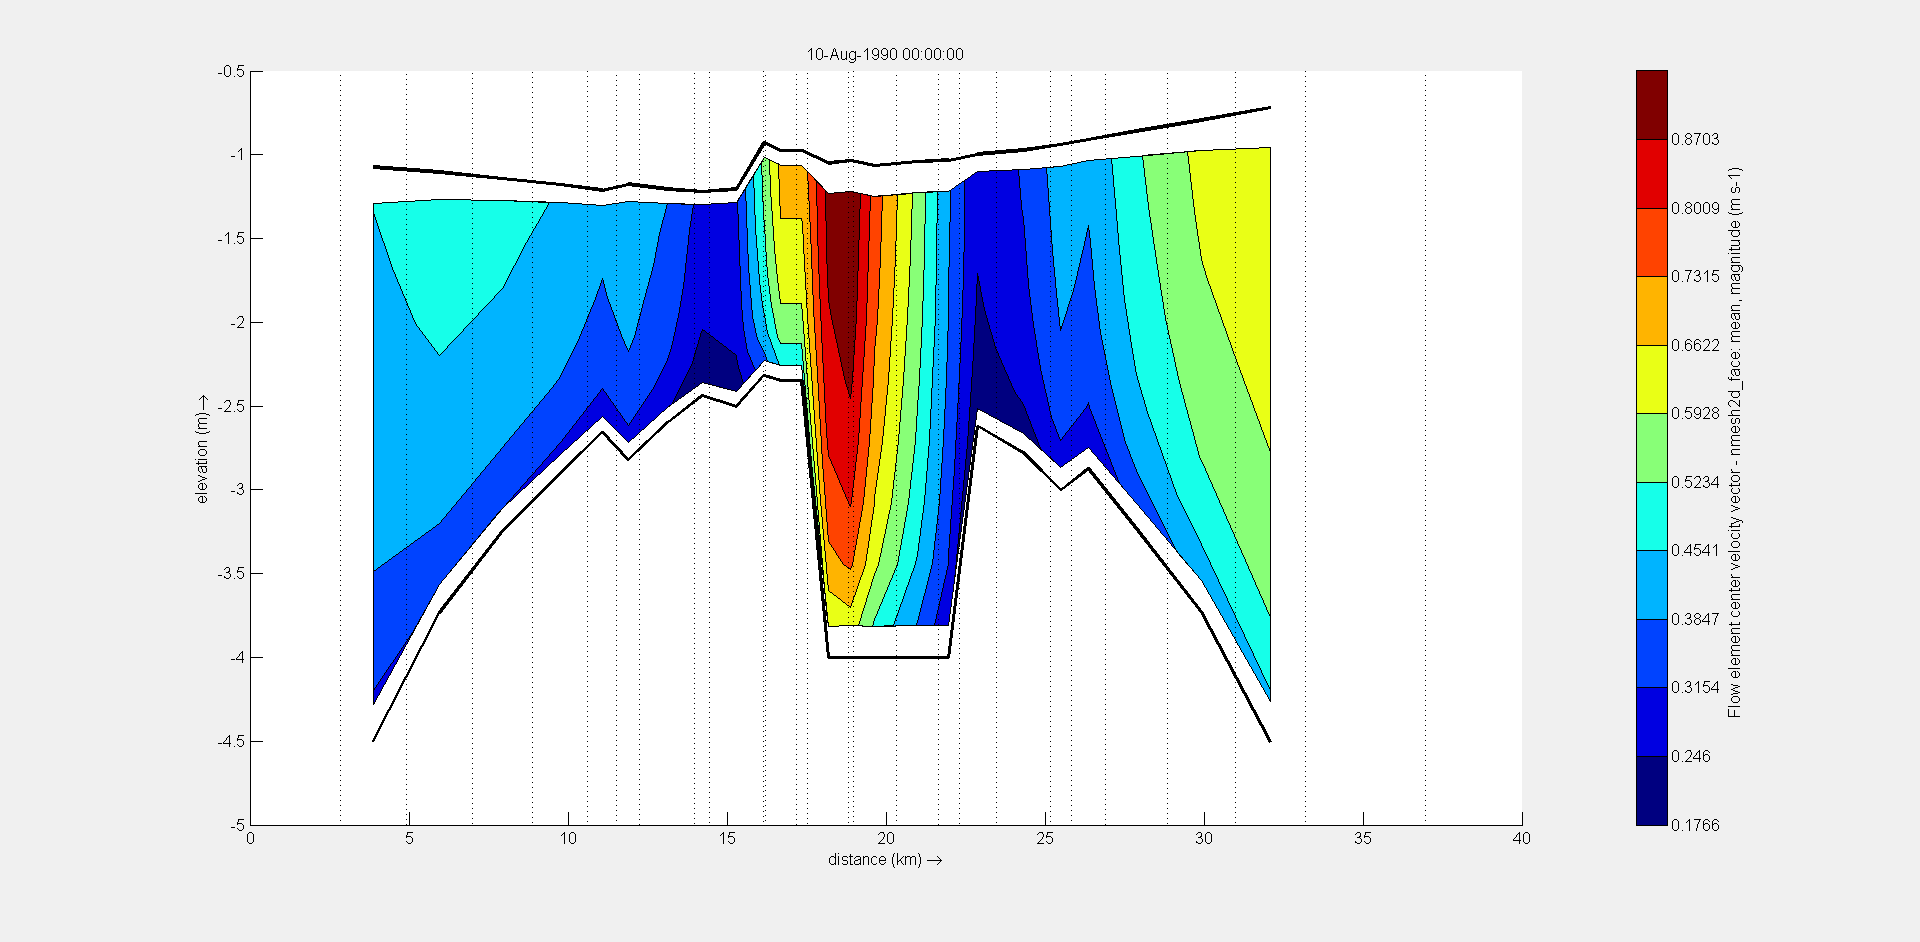
\includegraphics[width=\textwidth]{Ch06/VSliceScalarContours.png}}
\caption{Slice of the velocity magnitude along the line shown in \Fref{fig:VSliceScalarGridViewArbLine} using presentation type Contour Patches for the velocity and Linear for the water level and the bed level.}
\label{fig:VSliceScalarContours}
\end{figure}

\subsection{Vertical plot of tracks} \label{Subsec:VerticalTracks}
The pathways of particles that are transported in three dimensions can not only be visualized from above (see \Autoref{Subsec:MapTracks}) but also from the side.
In that case we don't take a slice of their paths (which would typically be limited to a small number of intersection points of the paths) but we intend to visualize a side view of the path from the XZ- or YZ-plane.
As for the topview the particle tracks may either be coloured uniformly, or shaded by some property e.g.~time or the co-ordinate perpendicular to the viewing plane.

\subsection{Vertical profile against time} \label{Subsec:ProfileTime}
This is the vertical version of the horizontal transect against time discussed in \Autoref{Subsec:TransectTime}.
The time is plotted along the horizontal axis, and the vertical co-ordinate along the vertical axis.
This is identical to a standard time series plot for e.g.~the water level (see \Autoref{Subsec:GraphTimeSeriesScalar|}) and water levels and vertical concentration profiles against time can indeed easily be combined in one plot.

%------------------------------------------------------------------------------
\section{3D Plots} \label{Sec:PlotStyle3D}
Although one could think of various generalizations of slices in 3D, \QUICKPLOT\ currently only distinguishes between two 3D plots: the 3D plot with X, Y and Z co-ordinates, and the 3D plot with the Z co-ordinate replaced by another quantity, such as the velocity magnitude or the water temperature.

\subsection{2D Surface in 3D} \label{Subsec:2DSurfaceIn3D}
This is the 3D visualization of a 2D surface.
The same data as visualized using the 2D map \Autoref{Subsec:MapScalar} now also visualized using the quantity as the vertical coordinate.
This plot option is not yet supported by \QUICKPLOT.
